\section{From Binary Join to Free Join}\label{sec:background}

\begin{figure}
  \begin{align*}
    Q_{\clubsuit}(x,a,b,c) \cd R(x,a),S(x,b),T(x,c).
  \end{align*}
  \begin{center}
    \begin{tabular}{c}
      \begin{lstlisting}[language=SQL, numbers=none]
SELECT * FROM R, S, T WHERE R.x = S.x AND S.x = T.x
\end{lstlisting}
    \end{tabular}
  \end{center}
  \begin{alignat*}{8}
    R & = & \set{(x_0, a_0)} & \cup & \{(x_1, a_i^l), & (x_2, a_i^r) &  & \mid i \in [1 \ldots n] & \} \\
    S & = & \set{(x_0, b_0)} & \cup & \{(x_2, b_i^l), & (x_3, b_i^r) &  & \mid i \in [1 \ldots n] & \} \\
    T & = & \set{(x_0, c_0)} & \cup & \{(x_3, c_i^l), & (x_1, c_i^r) &  & \mid i \in [1 \ldots n] & \}
  \end{alignat*}
  \caption{The clover query $Q_\clubsuit$, and an input instance.
    Note that $x_0$ is the only $x$-value in all three relations,
    therefore the only output tuple is $(x_0, a_0, b_0, c_0)$. }
  \label{fig:clover-query}
\end{figure}

\begin{figure}
  \includegraphics*[width=.6\linewidth]{clover-2.pdf}
  \caption{Visualization of the input relations to $Q_\clubsuit$.
    Each binary relation is represented as a set of edges on each side.
    The query $Q_\clubsuit$ looks for sets of 3 edges, one from each relation,
    that meet in the middle (there is only one such set, at the center of the figure).}
  \label{fig:clover-Visualization}
\end{figure}

In this section we introduce the \FJ framework.
Unlike our SIGMOD paper~\cite{10.1145/3589295} which defines \FJ from
the basic building blocks,
here we start from the traditional binary join
and gently massage it into the more general \FJ.
To keep the presentation intuitive,
we will be following an example instead of
defining the algorithm in full generality.
We refer the reader to our SIGMOD paper~\cite{10.1145/3589295}
for a more formal treatment.

\subsection{Basic Concepts and Notations}\label{sec:basic-concepts}

For simplicity we consider only {\em natural join} queries,
where all joins are equijoins, and all input relations
are joined over common attributes.
Such queries are also known as {\em conjunctive queries}
and can be written in ``Datalog notation'' as the following
example shows.

\begin{example} \label{ex:triangle}
  Consider SQL query in Figure~\ref{fig:clover-query}.
  The corresponding conjunctive query appears above it,
  where each of $R(x, a)$, $S(x, b)$, and $T(x, c)$
  is called a {\em body atom}, and $Q_\clubsuit(x, a, b, c)$
  the {\em head atom}.
\end{example}

It is often convenient to view a conjunctive query as
a hypergraph.  The \emph{query hypergraph} of $Q$ consists of vertices
$\mathcal{V}$ and edges $\mathcal{E}$, where the set of nodes
$\mathcal{V}$ is the set of variables occurring in $Q$, and the set of
hyperedges $\mathcal{E}$ is the set of body atoms in $Q$.
The hypergraph for $Q_\clubsuit$ has four vertices, each for
$x$, $a$, $b$, and $c$,
and three edges, each for $R(x, a)$, $S(x, b)$, and $T(x, c)$.
As standard, we
say that the query $Q$ is {\em acyclic} if its associated hypergraph
is $\alpha$-acyclic\footnote{The reader does not need to be familiar
  with definitions of acyclic queries to understand \FJ.}~\cite{DBLP:journals/jacm/Fagin83}.
Note that $Q_\clubsuit$ is acyclic,
while an example of a {\em cyclic} query is the ``triangle query'':
$$Q_\triangle(x, y, z) \cd U(x, y), V(y, z), W(z, x).$$
whose query hypergraph is a triangle.

We now introduce a notation to make pseudocode cleaner.
Inside a loop,
we will write \lstinline|m = M[x]?|
for looking up $x$ from the hash map $M$;
if $M$ contains $x$, we assign the result of the lookup
to $m$; otherwise, we \lstinline|continue| to the next iteration
of the enclosing loop.
In other words, the code fragments in Figure~\ref{fig:lookup-notation}
are equivalent.
\begin{figure}
  \begin{subfigure}[t]{0.5\linewidth}
    \begin{lstlisting}
for ...:
  m = M[x]?
  ...
\end{lstlisting}
  \end{subfigure}
  \begin{subfigure}[t]{.45\linewidth}
    \begin{lstlisting}
for ...:
  if x not in M: 
    continue
  else: 
    m = M[x]
    ...
\end{lstlisting}
  \end{subfigure}
  \caption{Example using the notation \lstinline|m = M[x]?|.
    The two code fragments are equivalent.}
  \label{fig:lookup-notation}
\end{figure}

% \subsection{Basic Concepts}\label{sec:basic-concepts}

% For simplicity we consider only {\em natural join} queries,
% where all joins are equijoins, and all input relations
% are joined over common attributes.
% Such queries are also known as {\em conjunctive queries}
% and can be written in ``Datalog notation'' as the following
% example shows.

% \begin{example} \label{ex:triangle} Consider the following SQL query:
%   \begin{lstlisting}[language=SQL]
% -- Schema: R(x,y), S(y,z), T(z,x)
% SELECT R.x, S.y, T.z FROM R, S, T 
%  WHERE R.y = S.y AND S.z = T.z AND T.x = R.x
% \end{lstlisting}
%   %
%   The corresponding conjunctive query is:
%   $$Q_{\triangle}(x,y,z) \cd R(x, y), S(y,z), T(z, x).$$
%   %
%   where each of $R(x, y)$, $S(y,z)$, and $T(z, x)$
%   is called a {\em body atom}, and $Q_\triangle(x, y, z)$
%   the {\em head atom}.
% \end{example}

% It is often convenient to view a conjunctive query as
% a hypergraph.  The \emph{query hypergraph} of $Q$ consists of vertices
% $\mathcal{V}$ and edges $\mathcal{E}$, where the set of nodes
% $\mathcal{V}$ is the set of variables occurring in $Q$, and the set of
% hyperedges $\mathcal{E}$ is the set of body atoms in $Q$.
% The hypergraph for $Q_\triangle$ is a triangle with three
% vertices $x, y$, and $z$ and three edges corresponding to
% $R(x, y)$, $S(y,z)$, and $T(z, x)$.
% For this reason we will refer to $Q_\triangle$ as the {\em triangle
%     query}.
% As standard, we
% say that the query $Q$ is {\em acyclic} if its associated hypergraph
% is $\alpha$-acyclic\footnote{The reader does not need to be familiar
%   with definitions of acyclic queries to understand \FJ.}~\cite{DBLP:journals/jacm/Fagin83}.


\subsection{Binary Join}\label{sec:binary-join}

\begin{figure*}
  \begin{subfigure}[t]{0.21\linewidth}
    \begin{lstlisting}[showlines=true]
for (x,a) in R:
  s = S[x]?
  for (x,b) in s:
    t = T[x]?
    for (x,c) in t:
      output(x,a,b,c)




\end{lstlisting}
    \caption{Binary \FJ.}
    \label{fig:bj-loop}
  \end{subfigure}
  \begin{subfigure}[t]{0.27\linewidth}
    \centering
    \begin{lstlisting}[showlines=true, numbers=none]
for i in 0..R.len():
  x = R.x[i]; a = R.a[i]
  s = S[x]? # s:x->[j]
  for j in s:
    x = S.x[j]; b = S.b[j]
    t = T[x]? # t:x->[k]
    for k in t:
      x = T.x[k]; c = T.c[k]
      output(x,a,b,c)

\end{lstlisting}
    \caption{Columnar storage.}
    \label{fig:column-loop}
  \end{subfigure}
  \begin{subfigure}[t]{0.25\linewidth}
    \centering
    \begin{lstlisting}[escapeinside={(*}{*)}]
for i in 0..R.len():
  x = R.x[i]; s = S[x]?
  for j in s:
   (* \underline{x = S.x[j];} *)t = T[x]?
    for k in t:
     (* \underline{x = T.x[k]} *)
      a = R.a[i]
      b = S.b[j]
      c = T.c[k]
      output(x,a,b,c)
\end{lstlisting}
    \caption{Late materialization.}
    \label{fig:late-materialization}
  \end{subfigure}
  \begin{subfigure}[t]{0.25\linewidth}
    \centering
    \begin{lstlisting}[
    showlines=true,
    numbers=none
]
for i in 0..R.len():
  x = R.x[i]; 
  s = S[x]?; t = T[x]?
  for j in s:
    for k in t:
      a = R.a[i]
      b = S.b[j]
      c = T.c[k]
      output(x,a,b,c)

\end{lstlisting}
    \caption{Late iteration.}
    \label{fig:factorized-loop}
  \end{subfigure}
  \caption{Execution of binary join for the clover query~\ref{fig:bj-loop},
    and three transformations.
    The first transformation~\ref{fig:column-loop} makes the algorithm work
    on column-wise storage instead of a row-wise one;
    the second transformation~\ref{fig:late-materialization} performs
    the classic late materialization optimization;
    the last one is another transformation that we call
    late iteration~\ref{fig:factorized-loop}.
  }
\end{figure*}

The standard approach to computing a natural join of multiple relations is
to compute one binary join at a time.  A {\em binary plan} is a binary
tree, where each internal node is a join operator $\Join$, and each
leaf node is one of the base tables $R_i$.
The plan is a \emph{left-deep linear plan}, or
simply left-deep plan, if the right child of every join is a leaf
node.  If the plan is not left-deep, then we call it \emph{bushy}.
For example, $(R \Join S) \Join (T \Join U)$ is a bushy plan, while
$((R \Join S) \Join T) \Join U$ is a left-deep plan.  We do not treat
specially right-deep or zig-zag plans, but simply consider them to be
bushy.

In this paper we consider only hash-joins, which are the most
common types of joins in database systems.
The standard way to execute a bushy plan is to
decompose it into a series of left-deep linear plans.  Every join node
that is a right child becomes the root of a new subplan, which is
first evaluated, and its result materialized, before the parent join
can proceed.  As a consequence, every binary plan, bushy or not,
becomes a collection of left-deep plans. We decompose bushy
plans in exactly the same way, and we will focus on left-deep linear
plans in the rest of this paper.  For example, the bushy plan
$(R \Join S) \Join (T \Join U)$ is converted into two plans:
$P_1 = T \Join U$ and $P_2 = (R \Join S) \Join P_1$; both are
left-deep plans.

To reduce clutter, we represent a left-deep plan
$(\cdots ((R_1 \Join R_2) \Join R_3) \cdots \Join R_{m-1}) \Join R_m$
as $[R_1, R_2, \ldots, R_m]$.  Evaluation of a left-deep plan is done
using pipelining.  The engine iterates over each tuple in the
left-most base table $R_1$; each tuple is probed in $R_2$; each of the
matching tuple is further probed in $R_3$, etc.


\begin{example}
  A possible left-deep linear plan for $Q_\clubsuit$ is $[R, S, T]$,
  which represents $\left(R(x,a) \Join S(x,b)\right) \Join T(x,c)$.  To execute
  this plan, we first build a hash table for $S$ keyed on $x$,
  where each $x$ maps to a vector of $(x,y)$ tuples,
  and a hash table for $T$ keyed on $x$, each mapped to a
  vector of $(x,c)$ tuples\footnote{When the relations are bags, then
    the hash table may contain duplicate tuples, or store separately
    the multiplicity.  We also note that the question what exactly to
    store in the hash table (e.g. copies of the tuples, or pointers to
    the tuple in the buffer pool) has been studied for a long time,
    see~\cite{DBLP:journals/csur/Graefe93}.}.
  Then the execution
  proceeds as shown in Figure~\ref{fig:bj-loop}.
  For each tuple $(x, a)$ in $R$, we first probe into the hash table for $S$
  using $x$ to get a vector of $(x, b)$ tuples.  We then loop over
  each $(x, y)$ and probe into the hash table for $T$ with $x$.
  Each successful probe will return a vector of $(x, c)$ tuples,
  and we output the tuple $(x, a, b, c)$ for each $(x, c)$.
  On the input instance in Figure~\ref{fig:clover-query}
  (visualized in Figure~\ref{fig:clover-Visualization}),
  this algorithm runs in time $\Omega(n^2)$.
\end{example}

\subsection{Columnar Storage and Late Materialization}\label{sec:late-materialization}
The first transformation we perform on the binary join algorithm
makes it work on column-wise storage instead of a row-wise one.
This is not yet an optimization because it likely will not improve the
performance, but this step serves as an important bridge to the next
optimizations.
As Figure~\ref{fig:column-loop} shows, in the outermost loop we
iterate over row indices instead of tuples.
For each row index $i$, we retrieve the $x$-value $R.x[i]$,
as well as the corresponding $a$-value $R.a[i]$.
The hash maps for $S$ and $T$ now map each $x$ to a vector of row indices,
so we next look up into the hash map for $S$ using $x$
to get a vector of $j$.
In the second loop, we retrieve the $x$-value and $b$-value
from $S$ for each $j$,
then probe into $T$ to get a vector of $k$.
Finally, we retrieve the $x$-value and $c$-value from $T$ for each $k$,
and output the tuple $(x, a, b, c)$.

A key inefficiency of the algorithm in Figure~\ref{fig:column-loop} is that,
although the query only outputs a single tuple $(x_0, a_0, b_0, c_0)$,
we still did a lot of work retrieving the different, $a$, $b$, and $c$ values
from their respective columns.
For example, since we iterate over the entire $R$ relation,
we retrieve all $2n+1$ $a$-values from $R.a$;
even worse, since $|R \bowtie S| = n^2 + 1$,
we will access $S.b[j]$ $O(n^2)$ times.
A better strategy is to {\em delay} the retrieval of these values
until we actually need them.
In this case, we can delay the retrieval of $a$, $b$, and $c$
until we are ready to output the tuple $(x, a, b, c)$.
This way we only need to access each of $R.a$, $S.b$, and $T.c$ once,
instead of $O(n^2)$ times.
This is precisely the classic {\em late materialization}
optimization~\cite{DBLP:conf/icde/AbadiMDM07} now implemented in
nearly all modern database systems.

\subsection{Late Iteration and Free Join}\label{sec:late-materialization}
We can go one step beyond late materialization and further optimize
the code in Figure~\ref{fig:late-materialization}.
The key observation is that, although we retrieve $x$ from the
different relations in each loop level,
{\em they have to be the same value} because $x$ is the join attribute!
This means we can remove the last two redundant retrievals of $x$
and reuse the value from the outermost loop,
which corresponds to removing the underlined code
in Figure~\ref{fig:late-materialization}.
At this point, we can see that the remaining body of the second loop,
\lstinline|t = T[x]?|,
does not depend on the loop variable $j$ at all.
We can therefore pull the lookup out of the loop,
resulting in the code in Figure~\ref{fig:factorized-loop}.
In other words, we {\em delay} the iteration over $s$
until after the lookup on $T$ succeeds.

Note that this final optimization has improved the asymptotic
run time of the algorithm:
although late materialization already saves a quadratic
number of accesses to the relation columns,
it still needs to iterate over $O(n^2)$ row indices,
because the first two loop levels essentially compute
the join $R \bowtie S$.
In contrast, the first loop level in Figure~\ref{fig:factorized-loop}
joins every tuple of $R$ with $S$ and $T$ at the same time,
and the entire algorithm now runs in $O(n)$ time.

At the moment, our optimizations may appear rather low-level and ad-hoc.
Taking a step back, we can understand the execution of
any join algorithm as a series of iterations and lookups.
The transformation from row-wise to column-wise storage
involves changing {\em what to iterate over} (row indices instead of tuples);
the late materialization optimization changes {\em what to look up}
and {\em when to look up} (look up row indices first, then retrieve values later);
finally, the late iteration optimization reorders the iterations and lookups.

While columnar storage and late materialization have become stables of
modern database systems,
the contribution of the \FJ framework is a new abstraction
to describe the ordering of iterations and lookups
that we call the \FJ plan.
The basic building blocks of a \FJ plan are
called {\em subatoms}, each of which is a subset of a relation schema.
%
\begin{definition}
  Given a relation schema $R(x_1, x_2, \ldots)$,
  a \emph{subatom} of $R$ is of the form $R(x_i, x_j, \ldots)$
  where $\set{x_i, x_j, \ldots} \subseteq \set{x_1, x_2, \ldots}$
\end{definition}
%
For example, given the relation $R$ with schema $R(x, y)$,
all of the following are valid subatoms: $R(), R(x), R(y), R(x, y)$.
A \FJ plan over a set of schemas is a sequence of groups,
where each group is a list of subatoms.
%
\begin{definition}
  Given a join query $Q$ over $R_1, R_2, \ldots$,
  a \FJ plan for $Q$ is of the form $[R_i(\mathbf{x}_i), R_j(\mathbf{x_j}), \ldots],
    [R_k(\mathbf{x_k}), \ldots], \ldots$ where each of
  $R_i(\mathbf{x_i}), R_j(\mathbf{x_j}), R_k(\mathbf{x_k}), \ldots$
  is a subatom over the schema of $R_i, R_j, R_k, \ldots$ respectively.
\end{definition}
%
Each group in a \FJ plan corresponds to a loop level.
At each loop level,
we iterate over tuples of the first subatom in the group,
and use the values to look up into the remaining subatoms.
For this reason, we will sometimes stylize a \FJ plan as follows
to emphasize the iterated subatom and reflect the loop nesting:
\begin{alignat*}{4}
   & [R_1        &  & (\mathbf{x_1})\mid R_2(\mathbf{x_2}), R_3(\mathbf{x_3}), \ldots] \\
   & \rightarrow &  & [R_4(\mathbf{x_4})\mid R_5(\mathbf{x_2}), \ldots]                \\
   &             &  & \rightarrow [R_6(\mathbf{x_6})\mid \ldots]
\end{alignat*}
%
% Not every \FJ corresponds to a valid execution plan.
% For a subatom $R_i(\mathbf{x}_i)$ after the first position,
% because it denotes a lookup, each variable in $\mathbf{x}_i$
% must be introduced by some earlier subatom that is iterated over.
%
\begin{example}
  The \FJ plan for the algorithm in Figure~\ref{fig:factorized-loop}
  is:
  \begin{alignat*}{4}
     & [R(         &  & x, a) \mid S(x), T(x)]   \\
     & \rightarrow &  & [S(b) \mid ]             \\
     &             &  & \rightarrow [T(c) \mid ]
  \end{alignat*}
  Although we only retrieve the value of $a$ in the innermost loop,
  each $a$-value one-to-one corresponds to each $i$,
  so the plan iterates over both $x$ and $a$ at the first level.
\end{example}
%
\begin{example}
  We can represent the binary join algorithm in Figure~\ref{fig:bj-loop}.
  with the \FJ plan:
  \begin{alignat*}{4}
     & [R(         &  & x, a) \mid S(x)]        \\
     & \rightarrow &  & [S(b) \mid T(x)]        \\
     &             &  & \rightarrow [T(c) \mid]
  \end{alignat*}
  if we ignore the redundant $x$ at the inner loop levels.
\end{example}
%
In fact, every left-linear binary join plan $[R_1, R_2, R_3, \ldots]$
can be represented by a \FJ plan:
\begin{alignat*}{4}
   & [R_1(       &  & \mathbf{x_1}) \mid &  & R_2(\mathbf{\mathbf{x_1} \cap \mathbf{x_2}})]                                      \\
   & \rightarrow &  & [R_2(              &  & \mathbf{x_2} \setminus \mathbf{x_1}) \mid R_3(\mathbf{x_2}\cap \mathbf{x_3})]      \\
   &             &  & \rightarrow        &  & [R_3(\mathbf{x_3} \setminus \mathbf{x_2}) \mid R_4(\mathbf{x_3}\cap \mathbf{x_4})] \\
   &             &  &                    &  & \vdots
\end{alignat*}
%
As we will see in Section~\ref{sec:other-optimizations},
we can also represent any \GJ algorithm with a \FJ plan.
\FJ therefore generalizes and unifies both binary join and \GJ.
However, the true power of \FJ is its ability to represent
algorithms like the one in Figure~\ref{fig:factorized-loop}
that are neither binary join nor \GJ.
Intuitively, a (linear) binary join plan says which {\em relation}
to process at each step,
and always processes one additional relation at a time.
A \GJ plan says which {\em variable} to process at each step,
and always processes one variable at a time.
A \FJ plan can process any number of relations and variables at a time.
As we show in Figure~\ref{fig:free-join-space}, this flexibilty allows \FJ
to represent a much larger space of algorithms,
leading to performance improvements beyond the existing algorithms.

\begin{figure}
  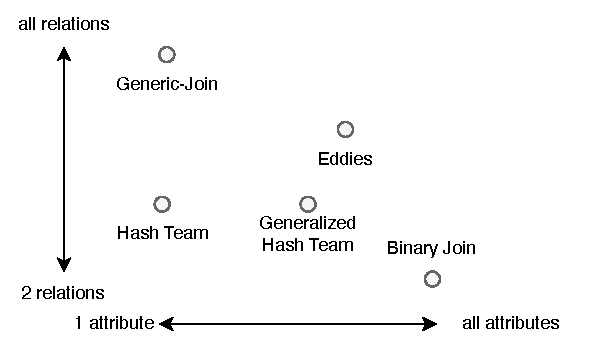
\includegraphics[width=.9\linewidth]{free-join.pdf}
  \caption{\FJ plans represent a design space of join algorithms
    that contains many existing algorithms.}
  \label{fig:free-join-space}
\end{figure}

\begin{figure*}
  \begin{subfigure}[t]{0.23\linewidth}
    \begin{lstlisting}
# [ R(x, y) | S(y) ]
# -> [ S(z) | T(z, x) ]

for (x,y) in R:
  s = S[y]? # S:y->[z]
  for z in s:
    if (z,x) in T:
      output(x,y,z)
\end{lstlisting}
    \caption{Plan equivalent to binary join.}
    \label{fig:bj-triangle}
  \end{subfigure}
  \begin{subfigure}[t]{0.25\linewidth}
    \begin{lstlisting}[numbers=none, showlines=true]
# [ R(x, y) | S(y), T(x) ]
# -> [ S(z) | T(z) ]

for (x,y) in R:
  s = S[y]?; t = T[x]?
  for z in s:
    if z in t:
      output(x,y,z)
\end{lstlisting}
    \caption{Another \FJ plan.}
    \label{fig:fj-triangle}
  \end{subfigure}
  \begin{subfigure}[t]{0.25\linewidth}
    \begin{lstlisting}[showlines=true]
# [ R(x, y) | S(y), T(x) ]
# -> [ S(z) $\cap$ T(z) ]

for (x,y) in R:
  s = S[y]?; t = T[x]?
  for z in s $\cap$ t:
    output(x,y,z)

\end{lstlisting}
    \caption{Plan with intersect ($\cap$).}
    \label{fig:inter-triangle}
  \end{subfigure}
  \begin{subfigure}[t]{0.25\linewidth}
    \begin{lstlisting}[showlines=true, numbers=none]
# [ R(y) $\cap$ S(y) ]
# -> [ S(z) $\cap$ T(z) ]
#    -> [ T(x) $\cap$ R(x) ]
for y in R.y $\cap$ S.y:
  for z in S[y] $\cap$ T.z:
    for x in T[z] $\cap$ R[y]:
      output(x,y,z)

\end{lstlisting}
    \caption{Plan equivalent to \GJ.}
    \label{fig:gj-triangle}
  \end{subfigure}
  \caption{Four different \FJ plans for $Q_\triangle$ and their execution.}
\end{figure*}

\subsection{Other Optimizations}\label{sec:other-optimizations}
In this section, we summarize a few additional optimizations
introduced in our SIGMOD paper~\cite{10.1145/3589295},
as well as relate \FJ to the \GJ algorithm.
To motivate these optimizations, we will follow the new example query
$Q_\triangle$ in Figure~\ref{fig:triangle-query},
and visualize an input instance in Figure~\ref{fig:triangle-input}.
Note $Q_\triangle$ is now a {\em cyclic} query, because its hypergraph
is a triangle with three vertices $x$, $y$, and $z$ and three edges
corresponding to $R(x, y)$, $S(y,z)$, and $T(z, x)$.

Let us first consider the algorithm in Figure~\ref{fig:bj-triangle}.
We show the \FJ plan in the comments atop the figure,
and note that it is equivalent to binary join.
To reduce clutter we will stick with a row-wise notation
while keeping in mind the underlying columnar storage.
We also remove redudant values from the hash maps;
for example, the hash map for $S$ in Figure~\ref{fig:bj-triangle}
now maps every $y$ to a vector of $z$ (instead of a vector of $(y, z)$).
The binary join algorithm first iterates over $(x, y)$-tuples in $R$,
using each $y$ to probe into $S$ to get a vector of $z$.
For each $z$, it then probes into $T$ to check if $(z, x)$ is in $T$,
and outputs the tuple $(x, y, z)$ if so.
This binary plan essentially computes the join $R \bowtie S$ first
before discarding tuples that do not join with $T$.
Because $R\bowtie T$ has size $O(n^2)$,
the algorithm runs in quadratic time.
Since the relations are symmetric, any binary join plan
will have the same asymptotic run time.

A different algorithm is shown in Figure~\ref{fig:fj-triangle}.
Here, as we iterate over tuples in $R$, we look up into $S$ and $T$
at the same time.
In other words we perform the late iteration optimization again,
pulling up lookups to discard tuples early.
However, this is not sufficient, because every tuple in $R$
does in fact join with both $S$ and $T$,
so the first loop level discards no tuples.
As the second loop level iterates over $s$,
we are in effect still computing the join $R \bowtie S$
which takes $O(n^2)$ time.
To overcome this inefficiency, we now introduce a new operator
called {\em intersection} ($\cap$).

\subsubsection{Intersection}
In contrast, the algorithm in Figure~\ref{fig:inter-triangle}
runs in linear time.
The small difference is that we have replaced the inner loop of
Figure~\ref{fig:fj-triangle}, which iterates over $s$,
with a loop iterating over the intersection of $s$ and $t$.
When we compute the intersection, we always iterate over the smaller
set while probing into the larger set.
To analyze the run time of this algorithm,
we first assume we have built a hash map for $S$,
mapping each $y$ to a {\em hash set} of $z$,
and similar for $T$.
Building each hash map takes linear time.
Then, as we iterate over $R$, we consider three cases:
\begin{enumerate}
  \item For the tuple $(x_0, y_0)$, $s = S[y_0] = \setof{z_i}{i \in [0, \ldots, n]} = T[x_0] = t = s \cap t$,
        so we may iterate over either $s$ or $t$ to compute $s \cap t$ in linear time.
  \item For each tuple $(x_0, y_i)\mid i > 0$, $t = T[x_0] \setof{z_i}{i \in [0, \ldots, n]}$ but
        $s = S[y_i] = \set{z_0}$, so we iterate over (the only element of) $s$
        and probe into $t$ to compute $s \cap t$.
        This takes constant time for each $y_i$, so for all $y_i$ the total time is linear.
  \item The case for tuple $(x_i, y_0)$ is symmetric to the previous case, so it also takes linear time.
\end{enumerate}
Overall, the algorithm in Figure~\ref{fig:inter-triangle} runs in linear time.
Another way to think about the intersection operation is to
understand it as dynamically reording the iterations and lookups:
to compute $s \cap t$, we switch between
the plans $[S(z) \mid T(z)]$ and $[T(z)\mid S(z)]$ depending on which one is smaller.

\subsubsection{\GJ}
We can now faithfully derive the \GJ algorithm as a special case of \FJ,
using the itersection operator.
Suppose an instance of \GJ follows the variable order $x_1, x_2, \ldots, x_n$.
The corresponding \FJ plan is:
\begin{alignat*}{4}
   & [R_1^1(     &  & x_1) \cap R_1^2(x_1) \cap \cdots]                    \\
   & \rightarrow &  & [R_2^1(x_2) \cap R_2^2(x_2) \cap \cdots]             \\
   &             &  & \vdots                                               \\
   &             &  & \rightarrow [R_n^1(x_n) \cap R_n^2(x_n) \cap \cdots]
\end{alignat*}
where $R_i^j$ is a relation that contains $x_i$ in its schema.
When computing a multiway intersection, we (dynamically) pick
the smallest set to iterate over and probe into the rest.
For any choice of the variable order,
the \GJ algorithm is guaranteed to run in worst-case
optimal time~\cite{DBLP:conf/icdt/Veldhuizen14,DBLP:conf/pods/000118,DBLP:conf/pods/NgoPRR12}.


\subsubsection{Lazy trie building}
To explain the algorithm in Figure~\ref{fig:fj-triangle} we assumed
to have pre-built hash maps for $S$ and $T$.
A more efficient strategy is to {\em lazily} construct parts of the data structures
as we iterate over the relations.
Specifically, we will only build the hash set for $s$ (or $t$)
right before we need to probe into it.
This way, we can avoid building a linear number of (singleton) hash sets
that we only need to iterate over.
In the full paper~\cite{10.1145/3589295} we describe a data structure,
called Column-oriented Lazy Trie (COLT), that generalizes this idea.

\begin{figure}
  $Q_\triangle \cd R(x, y), S(y, z), T(z, x).$
  \begin{center}
    \begin{tabular}{c}
      \begin{lstlisting}[language=SQL, numbers=none]
SELECT * FROM R,S,T -- R(x,y), S(y,z), T(z,x)
 WHERE R.y = S.y AND S.z = T.z AND T.x = R.x
\end{lstlisting}
    \end{tabular}
  \end{center}
  \begin{align*}
    R  = \setof{(x_0, y_i)}{y \in [0 \ldots n]} \cup \setof{(x_i, y_0)}{y \in [0 \ldots n]} \\
    S  = \setof{(y_0, z_i)}{y \in [0 \ldots n]} \cup \setof{(y_i, z_0)}{y \in [0 \ldots n]} \\
    T  = \setof{(z_0, x_i)}{y \in [0 \ldots n]} \cup \setof{(z_i, x_0)}{y \in [0 \ldots n]}
  \end{align*}
  \caption{The triangle query $Q_\triangle$, and an input instance.}
  \label{fig:triangle-query}
\end{figure}

\begin{figure}
  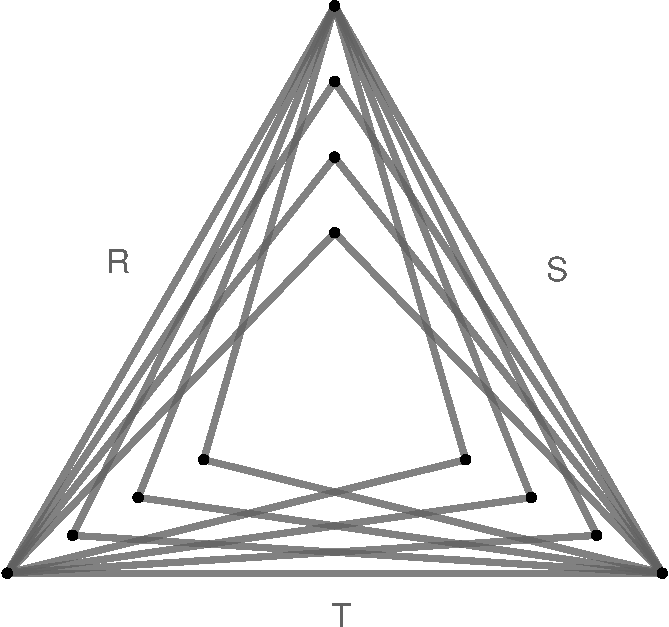
\includegraphics[width=.6\linewidth]{triangles-2.pdf}
  \caption{Visualization of input relations to $Q_\triangle$.
    Each relation is represented by a set of edges.
    The query $Q_\triangle$ looks for triangles formed by
    one edge from each relation (there are 10).}
  \label{fig:triangle-input}
\end{figure}

\begin{figure}
  \begin{lstlisting}
def join(plan, tuple, R, S, T, ...):
  if plan is empty: output(tuple)
  else:
    let [ R(xs) | S(ys), T(zs), ... ] = plan[0]
    for xs in R:
      r = R[xs]?; s = S[ys]?; t = T[zs]?; ...
      join(plan[1:], tuple ++ xs, r, s, t, ...)
\end{lstlisting}
  \caption{Recursive formulation of \FJ.}
  \label{fig:fj-recursive}
\end{figure}


\begin{figure}
  \begin{lstlisting}
def join(plan, tuple, R, S, T, ...):
  if plan is empty: output(tuple)
  else:
    let [ R(xs) | S(ys), T(zs), ... ] = plan[0]
    tup_rels = {} # map a partial tuple to sub-relations
    for xs_batch in R.iter_batch():
      for xs in xs_batch:
        r = R[xs]?; s = S[ys]?; t = T[zs]?; ...
        tup = tuple ++ xs
        tup_rels[tuple] = (r, s, t, ...)
    for (tup, rels) in tup_rels:
      join(plan[1:], tup, rels)
\end{lstlisting}
  \caption{Vectorized execution for \FJ.}
  \label{fig:vectorized-execution}
\end{figure}

\subsubsection{Vectorized Execution}\label{sec:vectorized-execution}
A simple way to implement \FJ is to use a recursive function,
as shown in Figure~\ref{fig:fj-recursive}.
For every group in the \FJ plan,
we iterate over the first subatom and probe into the remaining subatoms.
If all probes are successful, we append new values to the partial tuple,
and recursively call \lstinline|join| on the remaining plan and sub-relations.
This na\"ive implementation suffers from poor temporal locality:
in the body of the loop,
we probe into the same set of relations for each tuple.
But these probes are interrupted by the recursive
call at the end,
which is itself a loop interrupted by further recursive calls.

A simple way to improve locality is to perform a batch of probes
before recursing, just like the classic vectorized execution
for binary join.
As shown in Figure~\ref{fig:vectorized-execution},
we call \lstinline|iter_batch| to retrieve a batch of tuples from $R$.
For each tuple in a batch,
we probe into the relations to get the corresponding sub-relations.
If all probes are successful, we append new values to the partial tuple,
and pair the tuple with the respecitve sub-relations;
otherwise we continue onto the next tuple in the batch.
Finally, for each tuple that successfully probes into all relations,
we call \lstinline|join| recursively on the remaining plan.

% \subsection{\GJ}\label{sec:background:gj}

% \GJ was introduced in~\cite{DBLP:journals/sigmod/NgoRR13} and is the
% simplest worst-case optimal join algorithm.  It is based on the
% earlier Leapfrog Triejoin algorithm~\cite{DBLP:conf/icdt/Veldhuizen14}.
% %
% \GJ computes a join query through a series of nested
% loops, where each loop iterates over a {\em variable} (not a tuple).
% Concretely, \GJ chooses arbitrarily a variable $x$, computes the
% intersection of all $x$-columns of all relations containing $x$, and
% for each value $a$ in this intersection it computes the residual query
% $Q[a/x]$, where every relation $R$ that contains $x$ is replaced with
% $\sigma_{x=a}(R)$.  In pseudocode (where $\Pi_x (R_i)$ is the $x$-column of $R_i$):
% %
% \begin{lstlisting}[basicstyle=\ttfamily]
% def join(Q, tuple): # tuple is initially empty
%   if Q is empty: print(tuple)
%   else:
%     for a in $\bigcap_{i : x \in schema(R_i)} \Pi_x(R_i)$:
%       join(Q[a/x], tuple ++ [a])
% \end{lstlisting}
% %
% If the query $Q$ has $k$ variables, then there are $k$ nested loops in
% \GJ.  In the inner most loop, \GJ outputs the tuple of constants, one
% from each iteration.\footnote{For bag semantics, it multiplies their
%   multiplicities.}  We notice that a plan for \GJ consists of a total
% order of the variables of the query, which we denote as
% $[x_1, x_2, \ldots, x_k]$.  Assuming that the intersection above is
% done optimally (see below), the algorithm is provably
% worst-case-optimal, for any choice of the variable order.

% \begin{example}
%   Fig.~\ref{fig:background:gj} shows the execution of \GJ on the
%   query $Q_\triangle$, using the variable order $[x,y,z]$.  We denoted
%   $\Pi_x(R)$ by $R.x$, and denoted (with some abuse) $\sigma_{x=a}(R)$
%   by $R[a]$.
% \end{example}


% While binary joins use hash tables, an implementation of \GJ uses a
% \emph{hash trie}, one for each relation in the query.  The hash-trie
% is a tree, whose depth is equal to one plus the number of attributes
% of the relation, and where each node is either an empty leaf
% node,\footnote{For bag semantics, we store in the leaf the
%   multiplicity of the tuple.} or a hash map mapping each atomic value
% to another node.  We will call the \emph{level} of a node to be the
% distance from the root, i.e. the root has level 0, its children level
% 1, etc.  The hash-trie completely represents the relation: every
% root-to-leaf path corresponds precisely to one tuple in the relation.
% \GJ uses the hash-trie as follows.  In order to compute
% $\sigma_{x=a}(R)$, it simply probes the current hash table for the
% value $x=a$, and returns the corresponding child.  To compute an
% intersection $\Pi_x(R_1) \cap \Pi_x(R_2) \cap \cdots$, it selects the
% trie with the fewest keys, say $R_1$, then iterates over every value
% $a$ in the keys for $R_1$ and probes it in each of the hash-maps for
% $R_2, R_3, \ldots$; this is a provably optimal algorithm for the
% intersection.

% \begin{example}
%   Consider the query $Q_\triangle$ and the \GJ plan $[x, y, z]$.  We
%   first build a hash trie each for $R$, $S$, and $T$.  Each trie has
%   three levels including the leaf.  Level 0 of $R$ is keyed on $x$,
%   level 1 is keyed on $y$, level 2 contains empty leaf nodes, and
%   similarly for $S$ and $T$.  Consider again the pseudocode in
%   Figure~\ref{fig:background:gj}.  The first loop intersects level 0
%   of the $R$-trie and the $T$-trie.  For each value $a$ in the
%   intersection, we retrieve the corresponding children $R[a]$ and
%   $T[a]$ respectively; these are at level 1.  The second loop
%   intersects the hash map $R[a]$ (at level 1) with the level 0
%   hash-map of $S$.  For each value $b$ in the intersection it
%   retrieves the corresponding children (levels 2 and 1 respectively),
%   and, finally, the innermost loop intersects the $S$- and $T$-hash
%   maps (both at level 2), and outputs $(a,b,c)$ for each $c$ in the
%   intersection.  So far we have assumed set semantics; if the
%   relations have bag semantics, then we simply multiply the tuple
%   multiplicities on the leaves (level 3).
% \end{example}

% %%% The original \GJ algorithm was specified for set semantics,
% %%% however~\cite{DBLP:journals/pvldb/FreitagBSKN20} showed the algorithm
% %%% can be easily extended to bag semantics.  We therefore ignore the
% %%% difference between the two semantics for the rest of this paper.

% \subsection{Binary Join v.s. \GJ}
% Binary join and \GJ each have their own advantages and disadvantages.
% \GJ became popular because of its asymptotic performance guarantee:
% Ngo, R{\'{e}}, and Rudra~\cite{DBLP:journals/sigmod/NgoRR13} proved the algorithm is
% \emph{worst-case optimal} for \emph{any variable order}, in the sense
% that its run time is bounded by the largest possible size of its
% output, called AGM bound~\cite{DBLP:journals/siamcomp/AtseriasGM13}.
% For example, \GJ executes $Q_\triangle$ in time
% $\sqrt{|R|\cdot |S| \cdot |T|}$, which is $n^{3/2}$ when all relations
% have size $n$; in contrast, a binary join plan can take $\Omega(n^2)$.
% We note, however, that this formula does not include the preprocessing
% time needed to construct the tries.  For example, if $T$ is
% significantly larger than $R, S$, then the run time of \GJ is
% $\ll |T|$, yet during preprocessing \GJ needs to read the entire
% relation $T$.  On the other hand, binary join has been a staple of
% database systems for decades.  The hash table data structure is
% simpler than hash tries and is cheaper to build.  Techniques like
% vectorized execution and column-oriented layout have also made binary
% join practically efficient, but these optimizations have not been
% adapted for \GJ.  Binary join plans are known to be very sensitive to
% the choice of the optimizer: poor plans perform catastrophically
% bad~\cite{DBLP:journals/pvldb/LeisGMBK015}.  In contrast, although the
% runtime performance of \GJ does depend on the variable order, some
% researchers believe that \GJ is less sensitive to poor variable
% orders, in part because it is always theoretically optimal.


% %%% \subsection{Basic Concepts}\label{sec:basic-concepts}
% %%% 
% %%% First, we define relations under bag semantics:
% %%% 
% %%% \begin{definition}
% %%%   A \emph{relation} is a bag (multiset) of tuples.
% %%%   The number of values in a tuple is its \emph{arity}.
% %%%   Every tuple in the same relation has the same arity 
% %%%     which is also the arity of the relation.
% %%%   Each relation has a \emph{schema}, which is a tuple of distinct variables.
% %%%   The size of the schema is the same as the arity of the relation.
% %%% \end{definition}
% %%% 
% %%% For convenience, we sometimes refer to the schema of a tuple, 
% %%%   which is the schema of the relation holding that tuple.
% %%% We also associate each value in a tuple with a variable in the tuple's schema.
% %%% 
% %%% To simplify presentation we focus on queries involving only 
% %%%   natural joins in this paper, although our implementation 
% %%%   also supports standard relational algebra operations 
% %%%   like selection, projection and aggregation.
% %%% In other words, every query is a \emph{full conjunctive query}:
% %%% \begin{definition}
% %%%   A \emph{full conjunctive query} is a set of \emph{atom}s,
% %%%   where each atom is a relation name paired with a tuple of variables.
% %%%   The number of variables in each tuple is the same as the arity of the relation.
% %%%   We assume no two atoms share the same relation name, 
% %%%   and each variable appears at most once in the same atom.
% %%% \end{definition}
% %%% 
% %%% We handle a self-join of a relation $R$
% %%%   by creating a copy of $R$ and renaming it to $R'$.
% %%% This is the standard approach in database systems 
% %%%   that require each query plan to be a tree.
% %%% Without loss of generality,
% %%%   we assume each relation's schema coincides with 
% %%%   the variables of its atom in the query.
% %%% 
% %%% \begin{example}
% %%%   Consider the \emph{triangle query} over relations $R$, $S$, $T$:
% %%% $$Q_{\triangle} \cd R(x, y), S(y,z), T(x, z).$$
% %%% It is the same as the following SQL query:
% %%% \begin{lstlisting}[
% %%%     language=SQL,
% %%%     showspaces=false,
% %%%     basicstyle=\ttfamily\small,
% %%%     numbers=left,
% %%%     numberstyle=\tiny,
% %%%     commentstyle=\color{gray}
% %%%  ]
% %%% SELECT * FROM R, S, T -- schema: R(x,y), S(y,z), T(x,z)
% %%%  WHERE R.y = S.y AND S.z = T.z AND T.x = R.x
% %%% \end{lstlisting}
% %%% \end{example}
% %%% 
% %%% The precise definition of cyclic and acyclic queries 
% %%%   is not important for this paper,
% %%%   so we discuss them informally and briefly here.
% %%% Fix a conjunctive query $Q$.
% %%% The \emph{query hypergraph} of $Q$ consists of vertices $\mathcal{V}$
% %%%   and edges $\mathcal{E}$, 
% %%%   where each $v \in \mathcal{V}$ is a variable
% %%%   and each hyperedge $(v_1, \ldots, v_k) \in \mathcal{E}$
% %%%   is the relation whose atom has the variables $(v_1, \ldots, v_k)$.
% %%% A sufficient condition for a query to be acyclic is that 
% %%%   the query hypergraph is a tree.
% %%% $Q_\triangle$ is a \emph{cyclic} query, 
% %%%   whereas any chain query is acyclic, e.g. $Q \cd R(x,y), S(y, z), T(z,w).$
% %%% 
% %%% \subsection{Binary Join}\label{sec:binary-join}
% %%% Now we review relevant concepts for binary join, 
% %%%   including its data structures, query plan.
% %%% 
% %%% Binary join works over \emph{hash tables}:
% %%% 
% %%% \begin{definition}
% %%%   A \emph{hash table} for $R$ is a hash map where each key is a tuple, 
% %%%     and every key is mapped to a vector of tuples.
% %%% \end{definition}
% %%% 
% %%% A \emph{binary plan} specifies how to execute a query with binary join:
% %%% 
% %%% \begin{definition}
% %%%   A \emph{binary plan} is a binary tree where each leaf is a distinct relation.
% %%%   A \emph{left-deep linear plan} is a binary plan where every right-child of an internal node is a leaf.
% %%%   Alternatively, we can write every left-deep linear plan as a sequence of relation names.
% %%%   There is a unique leaf that is a left-child, and the relation of that leaf is called the \emph{left relation}.
% %%%   A binary plan that is not a left-deep linear plan is called a \emph{bushy plan}.
% %%% \end{definition}
% %%% 
% %%% By this definition, we consider both ``right-deep'' plans and ``zig-zag'' plans as bushy plans,
% %%%   and do not distinguish between them.
% %%% A standard relational database executes a bushy plan by decomposing it into a series of left-deep linear plans.
% %%% That is, for each leaf on the left, it traverses the binary tree bottom-up by going only to the left parent,
% %%%   and all the nodes visited form a left-deep linear plan.
% %%% Then we execute these plans starting with the right-most one, materializing the intermediate results as we go.
% %%% We omit a formal description of this process for brevity.
% %%% Our system decomposes bushy plans in exactly the same way,
% %%%   and we will focus on left-deep linear plans in the rest of this paper.
% %%% 
% %%% \begin{example}
% %%%   A possible left-deep linear plan for $Q_\triangle$ is $[R, S, T]$.
% %%% \end{example}
% %%% 
% %%% We assume the reader is familiar with how a left-deep linear plan executes,
% %%%   and only provide an informal example here.
% %%%   of binary join for a different query.
% %%% 
% %%% \begin{figure}
% %%%   \begin{subfigure}[b]{0.45\linewidth}
% %%% \begin{lstlisting}
% %%% for (x, y) in R:
% %%%   S = S[y]?
% %%%   for z in S:
% %%%     T = T[x,z]?
% %%%     for () in T:
% %%%       output(x, y, z)
% %%% \end{lstlisting}
% %%%     \caption{Binary join.}
% %%%     \label{fig:back-binary-join}
% %%%   \end{subfigure}
% %%%   \begin{subfigure}[b]{0.45\linewidth}
% %%%     \centering
% %%% \begin{lstlisting}
% %%% for x in R.x $\cap$ T.x:
% %%%   R = R[x]; T = T[x]
% %%%   for y in R.y $\cap$ S.y:
% %%%     S = S[y]
% %%%     for z in S.z $\cap$ T.z:
% %%%       output(x, y, z)
% %%% \end{lstlisting}
% %%%     \caption{\GJ.}
% %%%     \label{fig:back-gj}
% %%%   \end{subfigure}
% %%%   \Description[TODO]{TODO}
% %%%   \caption{Execution of binary join and \GJ for $Q_\triangle$.
% %%%   The notation \lstinline|S[y]?| performs a lookup on $S$ with the key $y$,
% %%%    and continues to the enclosing loop if the lookup fails.  }
% %%% \end{figure}
% %%% 
% %%% \begin{example}
% %%%   Given the query $Q_\triangle$ and the plan $[R, S, T]$,
% %%%     we first build a hash table for $S$ keyed on $y$,
% %%%     where each $y$ maps to a vector of $z$ values.
% %%%     Then we build a hash table for $T$ keyed on $x$ and $z$,
% %%%     each mapped to a vector of empty tuples\footnote{
% %%%       We store the vectors of empty tuples to enforce bag semantics.
% %%%       An efficient implementation may simply store a count of duplicates.
% %%%     }.
% %%%   The nested loops in Figure~\ref{fig:back-binary-join} show the execution 
% %%%     of binary join.
% %%%   For each tuple $t = (x, y)$ in $R$, 
% %%%     we first probe into the hash table for $S$ using $y$
% %%%     to get a vector of $z$ values.
% %%%   We then loop over each $z$ 
% %%%     and probe into the hash table for $T$ using $x$ and $z$. 
% %%%   Each successful probe will return a vector of empty tuples, 
% %%%     and we output the tuple $(x, y, z)$ for each empty tuple.
% %%% \end{example}
% %%% 
% %%% \subsection{\GJ}
% %%% This section reviews basics of \GJ,
% %%%   including the hash trie data structure, 
% %%%   the \GJ plan, 
% %%%   and the execution of \GJ.
% %%% 
% %%% The data structure \GJ uses is called the \emph{hash trie}, 
% %%%   defined recursively as follows:
% %%% 
% %%% \begin{definition}
% %%%   A \emph{hash trie} is either a leaf, 
% %%%     or a hash map where each key is a single value 
% %%%       and every key is mapped to a hash trie.
% %%% \end{definition}
% %%% 
% %%% A hash trie can be seen as a tree, where 
% %%%   the concepts of \emph{parent}, and \emph{child}
% %%%   are defined in the usual way.
% %%% 
% %%% \begin{definition}
% %%%  A trie is a \emph{root} if it has no parents;
% %%%   any trie that is not a root is a \emph{subtrie}.
% %%% The \emph{level} of a subtrie is its distance from the root,
% %%%   i.e., the root is at level 0.
% %%% \end{definition}
% %%% 
% %%% A trie can represent a relation, 
% %%%   where the $i$-th level of the trie 
% %%%   stores values of the $i$-th attribute of the relation.
% %%% All the values along each path from the root to a leaf form 
% %%%   a tuple in the relation.
% %%% 
% %%% Now we define the \GJ plan that specify how to execute a query with \GJ.
% %%% 
% %%% \begin{definition}
% %%%   Fix a query $Q$.
% %%%   A \GJ plan for $Q$ is a total ordering of the variables in $Q$.
% %%% \end{definition}
% %%% 
% %%% A \GJ plan is executed by a series of nested loops, 
% %%%   where each loop level processes one variable 
% %%%   by \emph{intersecting} multiple tries on that variable.
% %%% We omit a formal definition for brevity, 
% %%%   and instead provide an informal example.
% %%% 
% %%% \begin{example}
% %%%   Consider the query $Q_\triangle$ and the \GJ plan $[x, y, z]$.
% %%%   We first build a hash trie each for $R$, $S$, and $T$.
% %%%   Each trie has three levels including the leaf.
% %%%   The first two levels for $R$, $S$, and $T$ are 
% %%%     keyed on $(x,y)$, $(y,z)$, and $(x,z)$, respectively.
% %%%   The execution of \GJ over these tries is shown in Figure~\ref{fig:back-gj}.
% %%%   The first loop intersects the tries for $R$ and $T$ on their keys.
% %%%   For each value $x$ in the intersection, 
% %%%     we retrieve the subtries mapped to $x$ from $R$ and $T$ respectively.
% %%%   The second loop intersects the subtrie for $R$ with the trie for $S$ on $y$,
% %%%     and retrieves the subtrie mapped to $y$ from $S$.
% %%%   Finally, the innermost loop intersects the subtries for $S$ and $T$ on $z$,
% %%%     and outputs the tuple $(x, y, z)$ for each value $z$ in the intersection.
% %%% \end{example}
% %%% 
% %%% The original \GJ algorithm was specified for set semantics, 
% %%%   however~\cite{DBLP:journals/pvldb/FreitagBSKN20} showed
% %%%   the algorithm can be easily extended to bag semantics.
% %%% We therefore ignore the difference between the two semantics 
% %%%   for the rest of this paper.
% %%% 
% %%% \subsection{Binary Join v.s. \GJ}
% %%% Binary join and \GJ each have their own advantages and disadvantages.
% %%% \GJ became popular because of its asymptotic performance guarantee:
% %%%   \citet{DBLP:journals/sigmod/NgoRR13} proved the algorithm is 
% %%%   \emph{worst-case optimal}, in the sense that 
% %%%   its run time is bounded by the worst-case output size.
% %%% For example, if each of the three relations in $Q_\triangle$ has $n$ tuples,
% %%%   there can be at most $n^{3/2}$ tuples in the output, 
% %%%   and \GJ runs in $O(n^{3/2})$ time.
% %%% In contrast, a binary join plan can take $\Omega(n^2)$ time 
% %%%   to compute the same query.
% %%% On the other hand, binary join has been a staple of database systems for decades. 
% %%% The hash table data structure is simpler than hash tries and is cheaper to build.
% %%% Techniques like vectorized execution and column-oriented layout have also 
% %%%   made binary join practically efficient,
% %%%   but these optimizations have not been adapted for \GJ.
% %%% 